\chapter{Single population growth models}
\label{chap:single_pop_growth}



\section{Objectives}
We are given a table with the population census at different time intervals between a date $a$ and a date $b$, and want to get an expression for the population. This allows us to: 
\begin{itemize}
\item compute a value for the population at any time between the date $a$ and the date $b$ (\textbf{interpolation}),
\item predict a value for the population at a date before $a$ or after $b$ (\textbf{extrapolation}).
\end{itemize}

%\begin{figure}[htbp]
%\begin{center}
%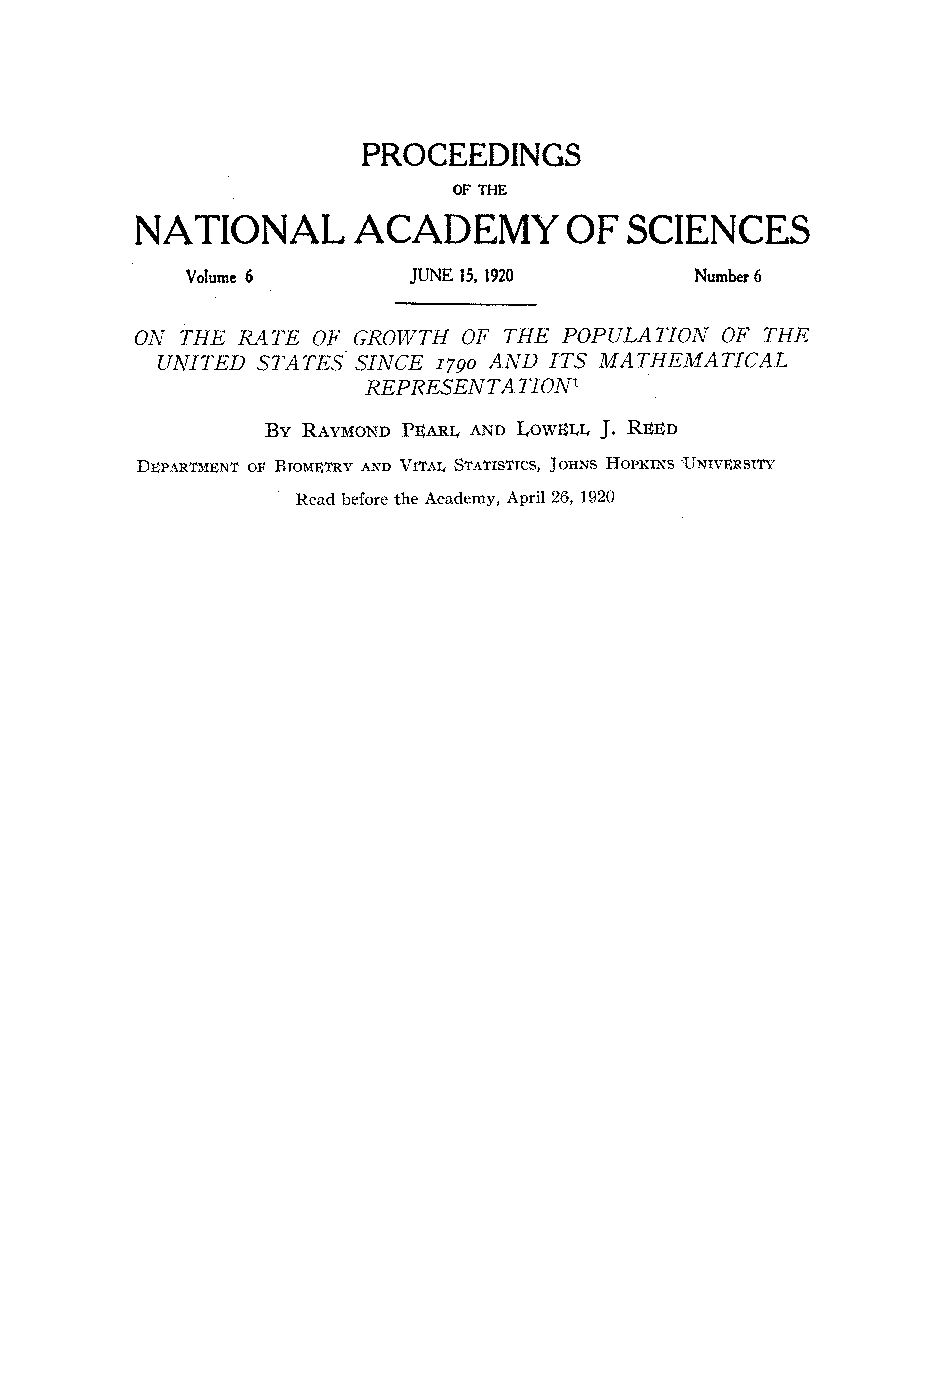
\includegraphics[width=0.7\textwidth]{../figs_02_population_growth/titre_PearlReed1920PNAS6}
%\end{center}
%\end{figure}

This was studied in a series of papers in the 1920-40's, mainly under the influence of Pearl and Reed \cite{PearlReed1920,PearlReed1930,PearlReedFish1940}.


\section{The data: US census}
% \begin{figure}[htbp]
% \begin{center}
% 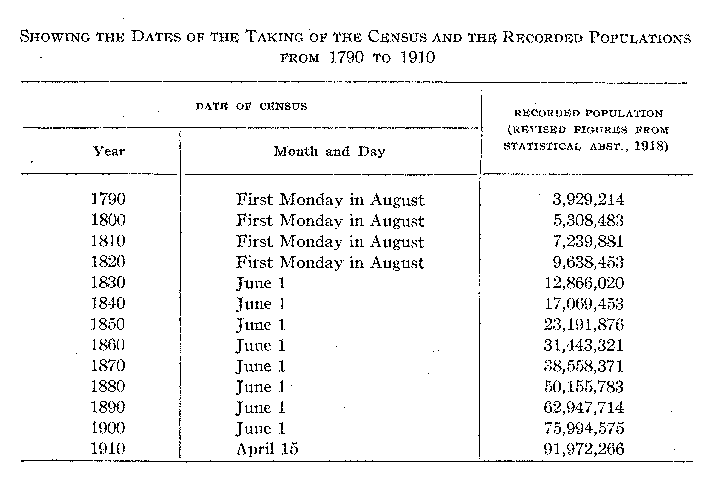
\includegraphics[width=0.8\textwidth]{../figs_02_population_growth/table_PearlReed1920PNAS6}
% \end{center}
% \end{figure}



\begin{table}[htbp]
\begin{center}
\begin{tabular}{cc}
Year & Population\\
& (millions) \\
\hline
1790 & 3.929 \\
1800 & 5.308 \\
1810 & 7.240 \\
1820 & 9.638 \\
1830 & 12.866 \\
1840 & 17.069 \\
1850 & 23.192 \\
1860 & 31.443 \\
1870 & 38.558 \\
1880 & 50.156 \\
1890 & 62.948 \\
1900 & 75.995 \\
1910 & 91.972 
\end{tabular}
\caption{The US population from 1790 to 1910. From Pearl and Reed
\cite{PearlReed1920}.}
\label{table:US_population_1790_1910}
\end{center}
\end{table}

Using MatLab (or Octave), create two vectors using commands such as
\begin{verbatim}
t=1790:10:1910;
\end{verbatim}
which creates the vector of time points, and 
\begin{verbatim}
P=[3929214,5308483,7239881,9638453,12866020, ...
    17069453,23191876,31443321,38558371,50155783, ...
    62947714,75994575,91972266];
\end{verbatim}
for corresponding population values ({\tt ...} indicates that the line continues below).
Then plot using
\begin{verbatim}
plot(t,P);
\end{verbatim}
\begin{center}
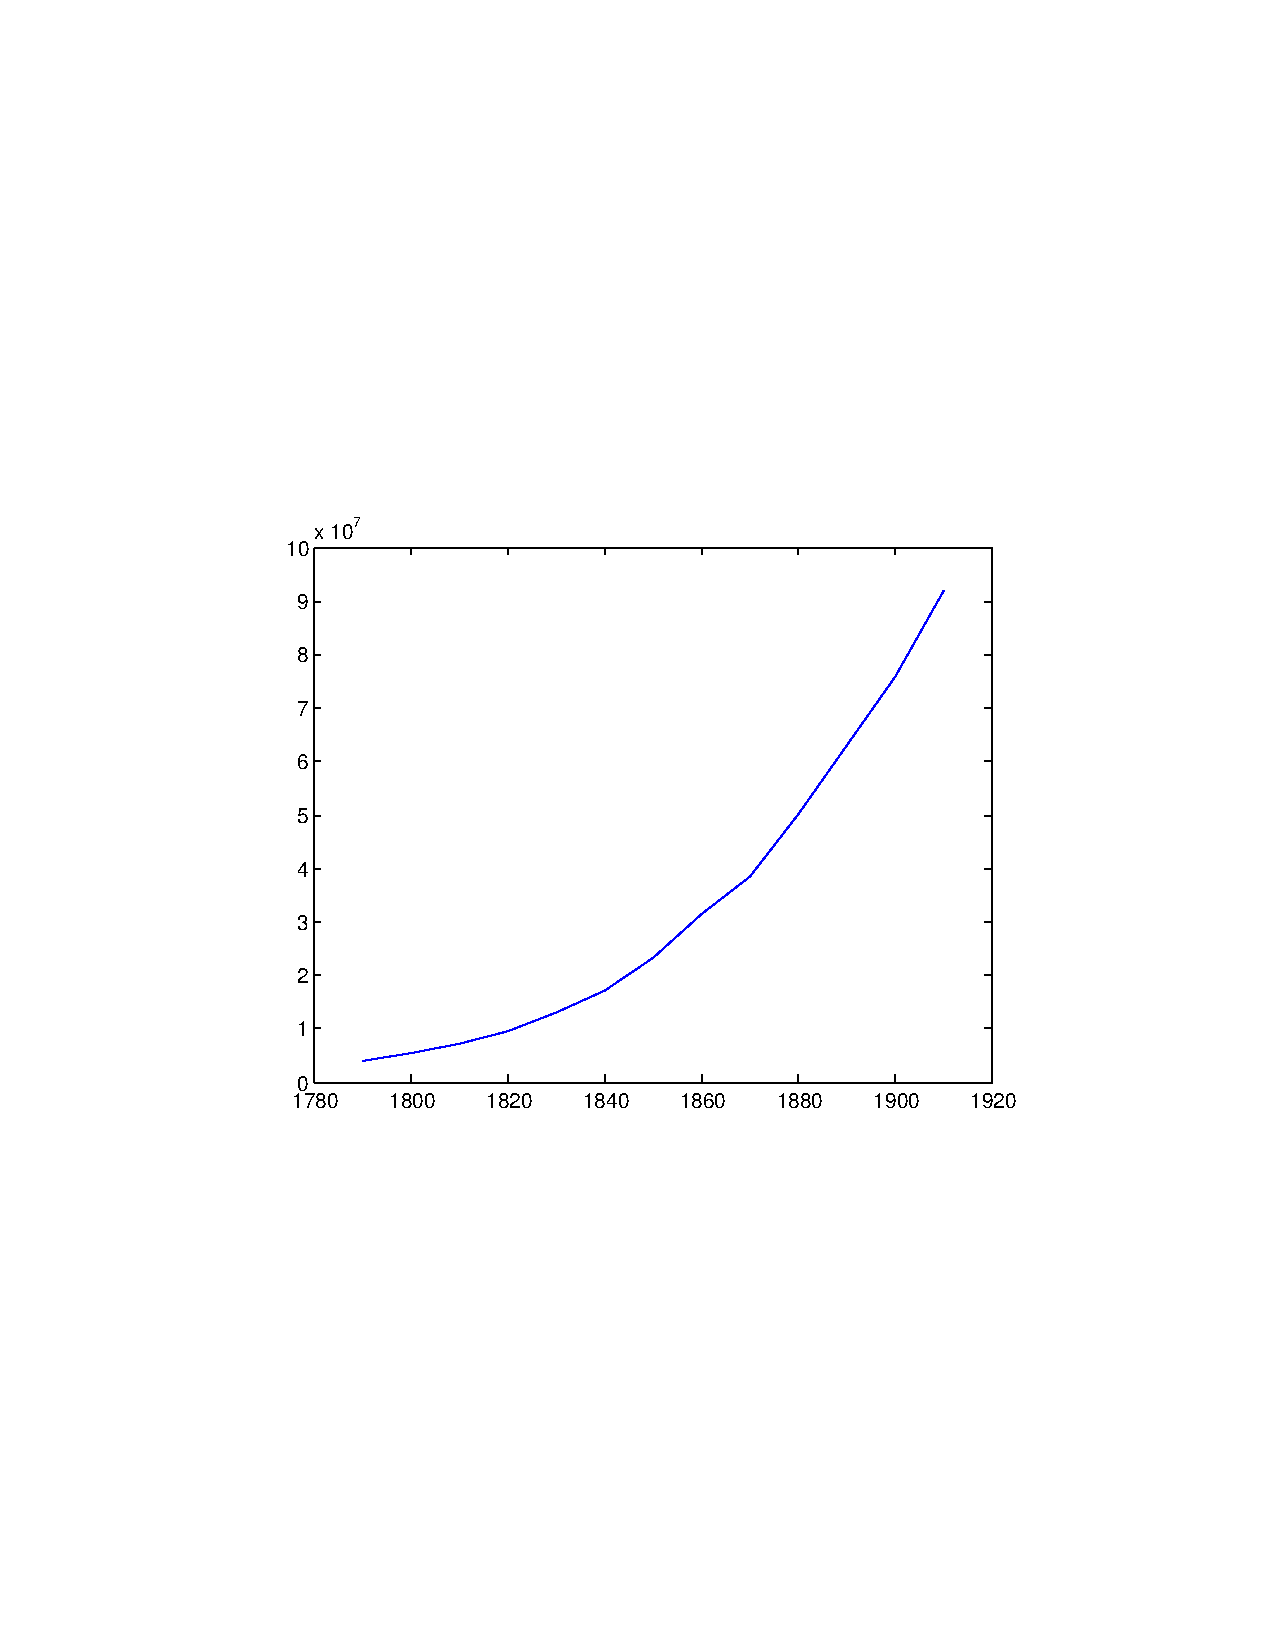
\includegraphics[width=0.5\textwidth]{../figs_02_population_growth/USpop_to1910}
\end{center}
To get points instead of a line, use the command
\begin{verbatim}
plot(t,P,'*');
\end{verbatim}
\begin{center}
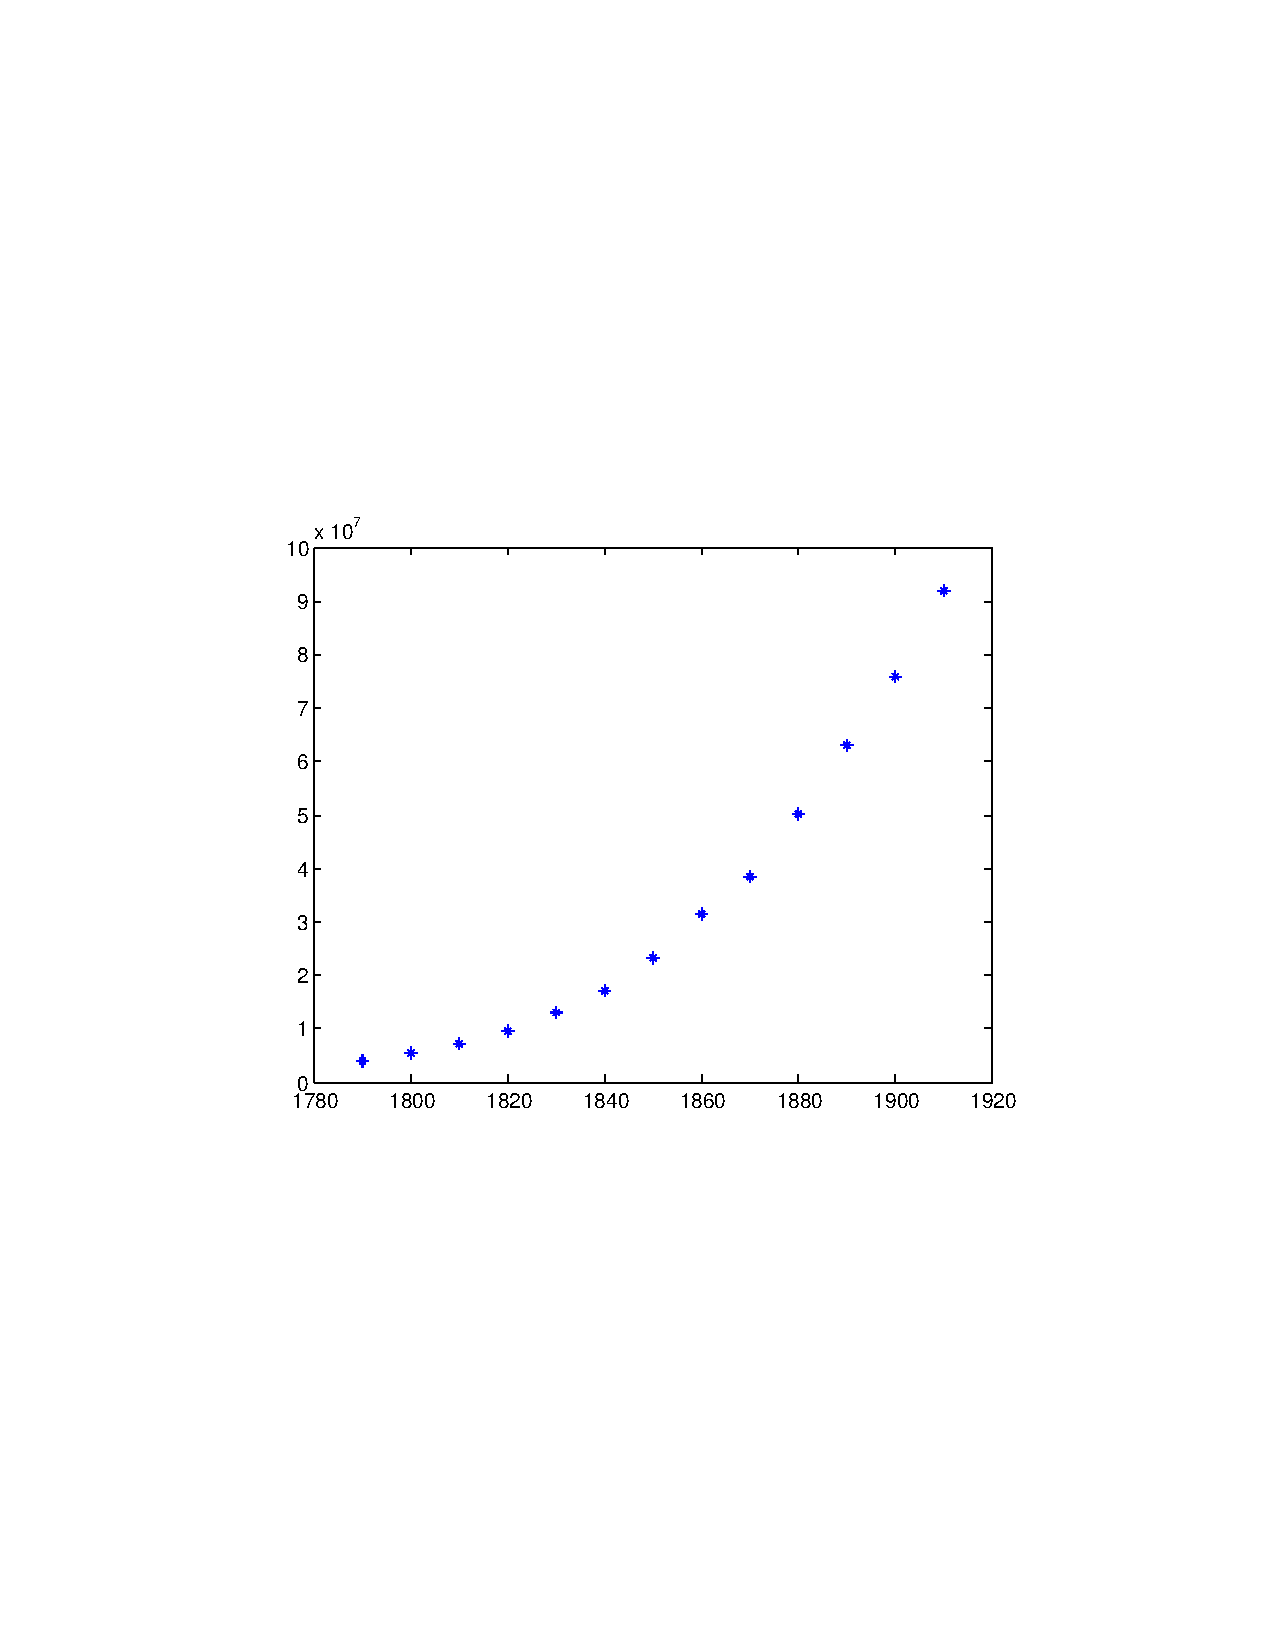
\includegraphics[width=0.5\textwidth]{../figs_02_population_growth/USpop_to1910_points}
\end{center}

\subsection{A quadratic curve?}
The curve looks like part of a parabola. So let us use nonlinear regression to fit a curve of the form
\[
P(t)=a+bt+ct^2
\]
to the data.
We proceed as follows.
There are 13 data points which we denote $(t_k,P_k)$ for $k=1,\ldots,13$. The objective of nonlinear regression is to find the values of $a,b,c$ such that
\[
S=\sum_{k=1}^{13} \left(P(t_k)-P_k\right)^2
\]
be minimal. This means that the values $a,b,c$ are such that the square of the distance between the the known points $(t_k,P_k)$ and those for corresponding times, $(t_k,P(t_k))=(t_k,a+bt_k+ct_k^2)$, is minimal. To emphasize the dependence of $S$ on the values of $a,b,c$, we denote it
\[
S(a,b,c)=\sum_{k=1}^{13} \left(a+bt_k+ct_k^2-P_k\right)^2.
\]
We have that $S(a,b,c)$ is minimal if (necessary condition) $\partial S/\partial a=\partial S/\partial b=\partial S/\partial c=0$, with
\begin{align*}
\frac{\partial S}{\partial a} &= 2\sum_{k=1}^{13}(a+bt_k+ct_k^2-P_k) \\
\frac{\partial S}{\partial b} &= 2\sum_{k=1}^{13}(a+bt_k+ct_k^2-P_k)t_k \\
\frac{\partial S}{\partial c} &= 2\sum_{k=1}^{13}(a+bt_k+ct_k^2-P_k)t_k^2.
\end{align*}
So we want
\begin{align*}
2\sum_{k=1}^{13}(a+bt_k+ct_k^2-P_k) &= 0\\
2\sum_{k=1}^{13}(a+bt_k+ct_k^2-P_k)t_k &= 0 \\
2\sum_{k=1}^{13}(a+bt_k+ct_k^2-P_k)t_k^2 &= 0,
\end{align*}
which we can simplify,
\begin{align*}
\sum_{k=1}^{13}(a+bt_k+ct_k^2-P_k) &= 0\\
\sum_{k=1}^{13}(a+bt_k+ct_k^2-P_k)t_k &= 0 \\
\sum_{k=1}^{13}(a+bt_k+ct_k^2-P_k)t_k^2 &= 0.
\end{align*}
Rearranging the system, we get
\begin{align*}
\sum_{k=1}^{13}(a+bt_k+ct_k^2) &= \sum_{k=1}^{13}P_k\\
\sum_{k=1}^{13}(at_k+bt_k^2+ct_k^3) &= \sum_{k=1}^{13}P_kt_k\\
\sum_{k=1}^{13}(at_k^2+bt_k^3+ct_k^4) &= \sum_{k=1}^{13}P_kt_k^2.
\end{align*}
After a bit of tidying up, and emphasizing the fact that the unknowns are $a,b,c$, we get
\begin{align*}
\left(\sum_{k=1}^{13}1\right)a+\left(\sum_{k=1}^{13}t_k\right)b+\left(\sum_{k=1}^{13}t_k^2\right)c &= \sum_{k=1}^{13}P_k \\
\left(\sum_{k=1}^{13}t_k\right)a+\left(\sum_{k=1}^{13}t_k^2\right)b+\left(\sum_{k=1}^{13}t_k^3\right)c &= \sum_{k=1}^{13}P_kt_k \\
\left(\sum_{k=1}^{13}t_k^2\right)a+\left(\sum_{k=1}^{13}t_k^3\right)b+\left(\sum_{k=1}^{13}t_k^4\right)c &= \sum_{k=1}^{13}P_kt_k^2.
\end{align*}
So we need to solve the linear system
\[
\begin{pmatrix}
13 & \sum\limits_{k=1}^{13}t_k & \sum\limits_{k=1}^{13}t_k^2 \\
\sum\limits_{k=1}^{13}t_k & \sum\limits_{k=1}^{13}t_k^2 & \sum\limits_{k=1}^{13}t_k^3 \\
\sum\limits_{k=1}^{13}t_k^2 & \sum\limits_{k=1}^{13}t_k^3 & \sum\limits_{k=1}^{13}t_k^4
\end{pmatrix}
\begin{pmatrix}
a\\ b\\ c
\end{pmatrix}
=
\begin{pmatrix}
\sum\limits_{k=1}^{13}P_k \\
\sum\limits_{k=1}^{13}P_kt_k \\
\sum\limits_{k=1}^{13}P_kt_k^2
\end{pmatrix}.
\]
With MatLab (or Octave), getting the values is easy.
\begin{itemize}
\item To apply an operation to every element in a vector or matrix, prefix the operation with a dot, hence
\begin{verbatim}
 t.^2;
\end{verbatim}
gives, for example, the vector with every element $t_k$ squared. 
\item Also, the function {\tt sum} gives the sum of the entries of a vector or matrix.
\item When entering a matrix or vector, separate entries on the same row by {\tt ,} and create a new row by using {\tt ;}.
\end{itemize}
Thus, to set up the problem in the form of solving $Ax=b$, we need to do the
following:
\begin{verbatim}
format long g;
A=[13,sum(t),sum(t.^2);sum(t),sum(t.^2),sum(t.^3);...
sum(t.^2),sum(t.^3),sum(t.^4)];
b=[sum(P);sum(P.*t);sum(P.*(t.^2))];
\end{verbatim}
The {\tt format long g} command is used to force the display of digits (normally, what is shown is in ``scientific'' notation, not very informative here). 

Then, solve the system using
\begin{verbatim}
A\b
\end{verbatim}
We get the following output:
\begin{verbatim}
>> A\b
Warning: Matrix is close to singular or badly scaled.
         Results may be inaccurate. RCOND = 1.118391e-020.

ans =
        22233186177.8195
        -24720291.325476
        6872.99686313725
\end{verbatim}
(note that here, Octave gives a solution that is not as good as this one, provided by MatLab).


\subsection{Checking our results for the quadratic}
Thus
\[
P(t)=22233186177.81-24720291.32t+6872.99t^2
\]
To see what this looks like,
\begin{verbatim}
plot(t,22233186177.81-24720291.32.*t+6872.99.*t.^2);
\end{verbatim}
(note the dots before multiplication and power, since we apply this function to every entry of $t$).
In fact, to compare with original data:
\begin{verbatim}
plot(t,22233186177.81-24720291.32.*t+6872.99.*t.^2,t,P,'*');
\end{verbatim}
\begin{figure}[htbp]
\begin{center}
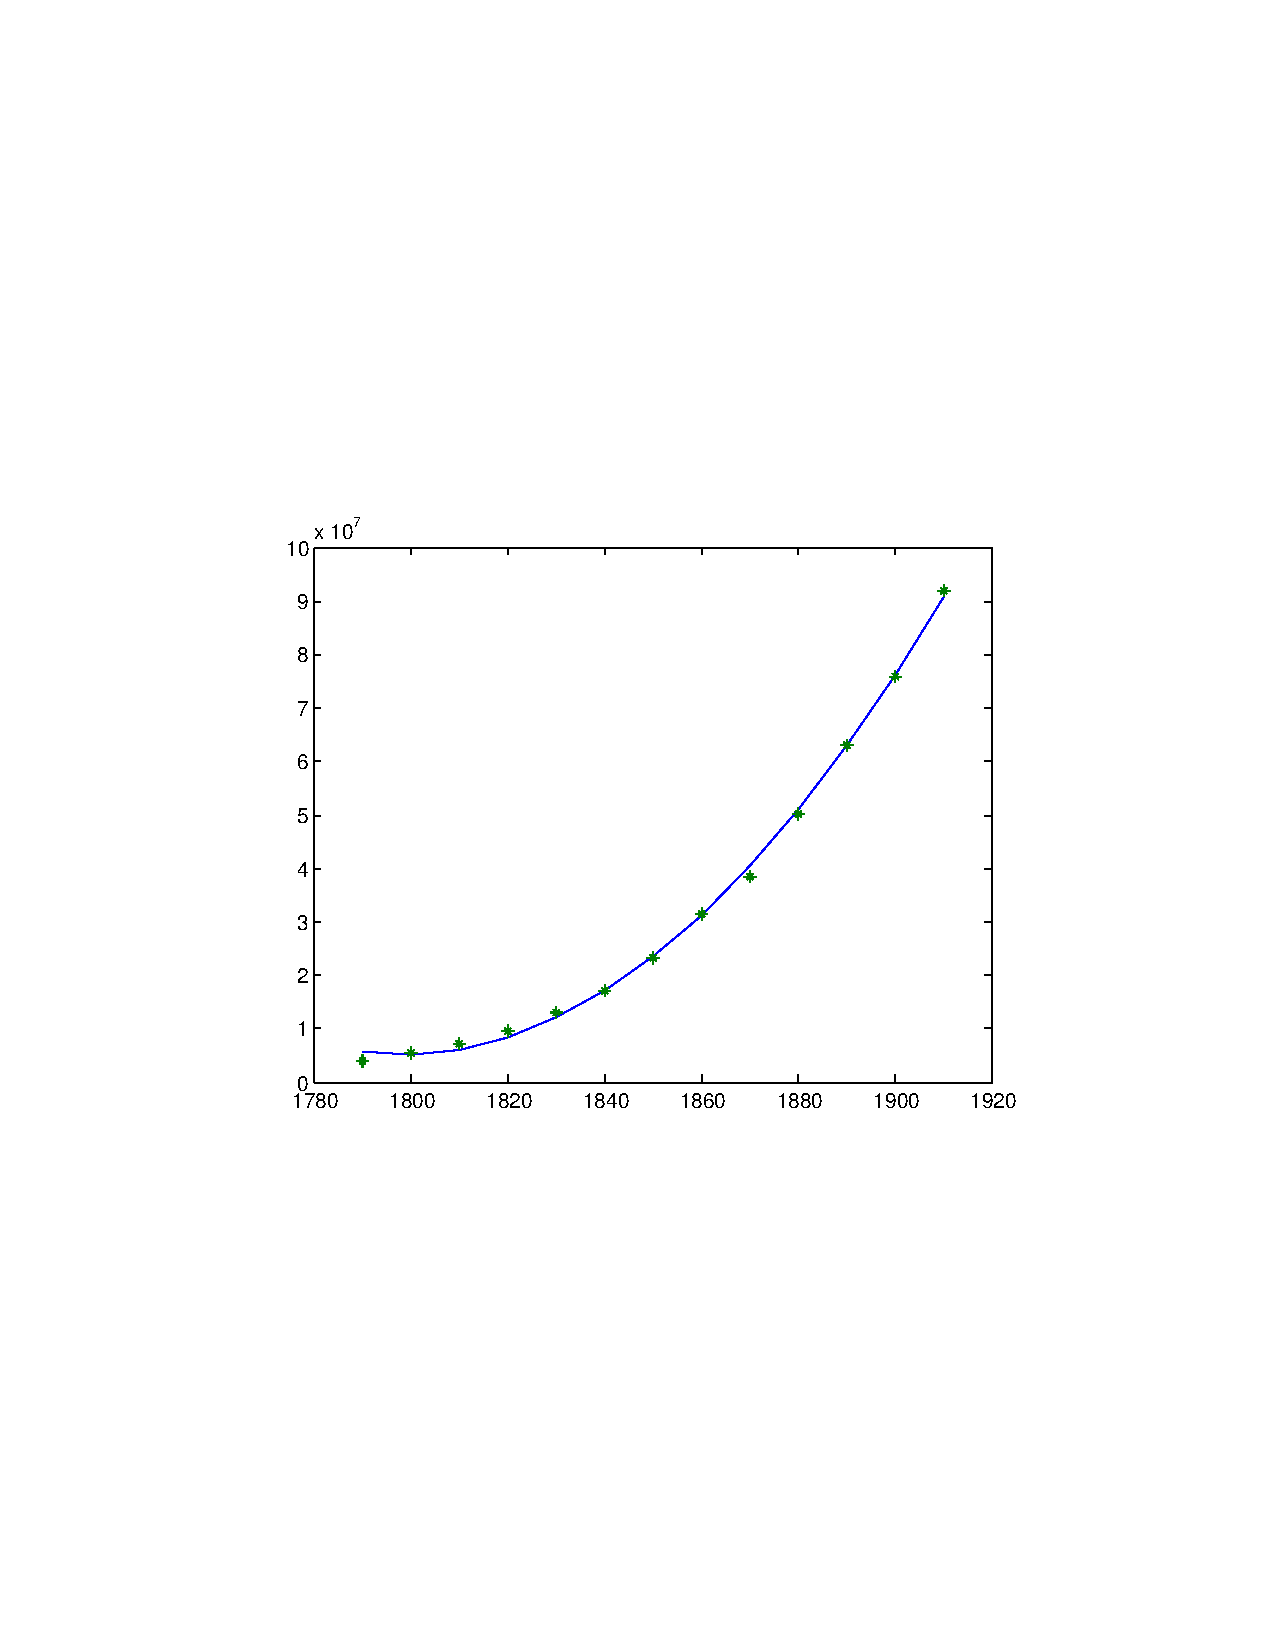
\includegraphics[width=0.5\textwidth]
{../figs_02_population_growth/quadratic_fit}
\end{center}
\end{figure}




Now we want to generate the table of values, to compare with the true values and thus compute the error. To do this, we can proceed directly:
\begin{verbatim}
computedP=22233186177.81-24720291.32.*t+6872.99.*t.^2;
\end{verbatim}
We get
\begin{verbatim}
computedP =
 Columns 1 through 4:
      5633954.39      5171628.52      6083902.03    8370774.90
 Columns 5 through 8:
      12032247.15      17068318.78      23478989.77    31264260.14
 Columns 9 through 12:
       40424129.88      50958598.99      62867667.48    76151335.34
 Column 13:
      90809602.57
\end{verbatim}

We can also create an \textbf{inline} function
\begin{verbatim}
f=inline('22233186177.81-24720291.32.*t+6872.99.*t.^2')
f =
     Inline function:
     f(t) = 22233186177.81-24720291.32.*t+6872.99.*t.^2
\end{verbatim}
This function can then easily be used for a single value
\begin{verbatim}
octave:24> f(1880)
ans =     50958598.9969215
\end{verbatim}
as well as for vectors.

(Recall that $t$ has the dates; $t$ in the definition of the function is a dummy
variable, we could have used another letter-.)
\begin{verbatim}
octave:25> f(t)
ans =
 Columns 1 through 4:
      5633954.39      5171628.52      6083902.03    8370774.90
 Columns 5 through 8:
      12032247.15      17068318.78      23478989.77    31264260.14
 Columns 9 through 12:
       40424129.88      50958598.99      62867667.48    76151335.34
 Column 13:
      90809602.57
\end{verbatim}
Form the vector of errors, and compute sum of errors squared:
\begin{verbatim}
octave:26> E=f(t)-P;
octave:27> sum(E.^2)
ans =     12186176863781.4
\end{verbatim}
Quite a large error (12,186,176,863,781.4), which is normal since we have used actual numbers, not thousands or millions of individuals, and we are taking the square of the error.

To present things legibly, one way is to put everything in a matrix..
\begin{verbatim}
M=[P;f(t);E;E./P];
\end{verbatim}
This matrix will have each type of information as a row, so to display it in the form of a table, show its transpose, which is achieved using the function {\tt transpose} or the operator $'$.
\begin{verbatim}
M'
ans =
 3929214      5633954.39      1704740.39     0.43
 5308483      5171628.52     -136854.47     -0.02
 7239881      6083902.03     -1155978.96    -0.15
 9638453      8370774.90     -1267678.09    -0.13
12866020      12032247.15     -833772.84   -0.06
17069453      17068318.78     -1134.21  -6.644728828e-05
23191876      23478989.77      287113.77    0.01
31443321      31264260.14     -179060.85  -0.00569471832254123
38558371      40424129.88      1865758.88    0.04
50155783      50958598.99      802815.99    0.01
62947714      62867667.48     -80046.51  -0.00127163502018304
75994575      76151335.34      156760.34   0.00206278330494212
91972266      90809602.57     -1162663.42    -0.01
\end{verbatim}


\frame{\frametitle{Now for the big question...}
How does our formula do for present times?
\begin{verbatim}
f(2006)
ans =     301468584.066013
\end{verbatim}
Actually, quite well: 301,468,584, compared to the 298,444,215 July 2006 estimate, overestimates the population by 3,024,369, a relative error of approximately 1\%.
}

\frame{\frametitle{The US population from 1790 to 2000 (revised numbers)}
\begin{center}
\begin{tabular}[t]{ccc}
\begin{tabular}{cc}
Year & Population\\
& (millions) \\
\hline
1790 & 3.929 \\
1800 & 5.308 \\
1810 & 7.240 \\
1820 & 9.638 \\
1830 & 12.866 \\
1840 & 17.069 \\
1850 & 23.192 \\
1860 & 31.443 \\
1870 & 38.558 \\
1880 & 50.156 \\
1890 & 62.948
\end{tabular} 
&\quad &
\begin{tabular}{cc}
Year & Population \\
& (millions) \\
\hline
1900 & 76.212 \\
1910 & 92.228 \\
1920 & 106.021 \\
1930 & 123.202 \\
1940 & 132.164 \\
1950 & 151.325 \\
1960 & 179.323 \\
1970 & 203.302 \\
1980 & 226.542 \\
1990 & 248.709 \\
2000 & 281.421
\end{tabular}
\end{tabular}
\end{center}
}

\subsection{Other similar approaches -- The logistic curve}
Pritchett \cite{Pritchett1891} tried
\[
P=a+bt+ct^2+dt^3,
\]
using data from 1790 to 1880 (inclusive).
%We have done this one, and found it to be quite good too.
Pearl and Reed, in \cite{PearlReed1920}, start by comparing the results of \cite{Pritchett1891} with those found by using 
\[
P(t)=a+bt+ct^2+d\ln t.
\]
They find
\[
P(t)=9,064,900-6,281,430t+842,377t^2+19,829,500\ln t.
\]
and a cumulative error ($S$) half of that of Pritchett.
They then try
\[
P(t)=\frac{be^{at}}{1+ce^{at}}
\]
or
\begin{equation}\label{eq:logistic_curve}
P(t)=\frac{b}{e^{-at}+c}.
\end{equation}
They find
\[
P(t)=\frac{2,930.3009}{e^{-0.0313395t}+0.014854}.
\]


\section{The ODE logistic equation}
\label{sec:ODE_logistic}

The \emph{logistic curve} \eqref{eq:logistic_curve} is the solution to an \emph{ordinary differential equation} called the \textbf{logistic equation}.
This equation was introduced by Pierre-Fran\c{c}ois Verhulst
(1804-1849) \cite{Verhulst1838,Verhulst1845}.
The idea is to represent a population evolving subject to the following effects:
\begin{itemize}
\item birth, at the \textbf{per capita} rate $b$,
\item death, at the \textbf{per capita} rate $d$,
\item competition of individuals with other individuals reduces their ability to survive, resulting in death.
\end{itemize}
This gives
\[
N'=bN-dN-\textrm{competition}.
\]
Competition describes the mortality that occurs when two individuals meet:
\begin{itemize}
\item
In chemistry, if there is a concentration $X$ of one product and $Y$ of another product, then $XY$, called \textbf{mass action}, describes the number of interactions of molecules of the two products.
\item
Here, we assume that $X$ and $Y$ are of the same type (individuals). So there are $N^2$ contacts.
\item 
These $N^2$ contacts lead to the death of individuals at the rate $c$.
\end{itemize}
Therefore, the \textbf{logistic} equation is
\begin{equation}\label{eq:ODE_logistic_second_form}
N'=bN-dN-cN^2.
\end{equation}
Rewriting this equation as
\[
N'=(b-d)N-cN^2,
\]
we see that 
\begin{itemize}
\item $b-d$ is the rate at which the population increases (or decreases) in the absence of competition. It is called the \textbf{intrinsic growth rate} of the population.
\item $c$ is the rate of \textbf{intraspecific} competition. The prefix \textbf{intra} refers to the fact that the competition is occurring between members of the same species, that is, within the species.\newline
[We will see later examples of \textbf{interspecific} competition, that is, between different species.]
\end{itemize}
Factor out an $N$ in \eqref{eq:ODE_logistic_second_form}, giving
\[
N'=\bigl((b-d)-cN\bigr)N.
\]
This gives us the original interpretation of the logistic equation, since, writing
\[
\frac{N'}N=(b-d)-cN,
\]
we have $N'/N$, the \textbf{per capita growth rate} of $N$, given by a constant, $b-d$, minus a \textbf{density dependent inhibition} factor, $cN$.

But the form \eqref{eq:ODE_logistic_second_form} is not the most well known form of the logistic equation. To obtain the most frequently used form, we transform \eqref{eq:ODE_logistic_second_form} as follows:
\begin{align*}
N' &= (b-d)N-cN^2\\
&= \bigl((b-d)-cN\bigr)N \\
&= \left(r-\frac rr cN\right)N,\quad\textrm{setting }r=b-d \\
&= rN\left(1-\frac crN\right) \\
&= rN\left(1-\frac NK\right),
\end{align*}
with
\[
\frac cr=\frac 1K.
\]
So, using the change of variables 
\[
(r,K)\leftrightarrow\left(b-d,\frac{b-d}c\right),
\]
we transform \eqref{eq:ODE_logistic_second_form} into the commonly used form
\begin{equation}\label{eq:ODE_logistic}
N'=rN\left(1-\frac NK\right),
\end{equation}
The parameter $r$ is the \textbf{intrinsic growth rate}, $K$ is the \textbf{carrying capacity}.
There are three ways to tackle this equation:
\begin{enumerate}
\item The equation is separable. [explicit method]
\item The equation is a Bernoulli equation. [explicit method]
\item Use qualitative analysis.
\end{enumerate}

\subsection{Solving the logistic as a separable equation}
\subsection{Solving the equation as a Bernoulli equation}

\subsection{Qualitative analysis of the logistic equation}
We study \eqref{sec:ODE_logistic}.
For this, write
\[
f(N)=rN\left(1-\frac NK\right),
\]
and consider the initial value problem (IVP) 
\begin{equation}\label{ivp:logistic_ode}
\begin{aligned}
N' &= f(N)\\
N(0) &= N_0\geq 0.
\end{aligned}
\end{equation}
The function $f$ is $C^1$ (differentiable with continuous derivative) so solutions to \eqref{ivp:logistic_ode} exist and are unique, by virtue of Theorem~\ref{th:existence_uniqueness_Cauchy}.
\textbf{Equilibria} of \eqref{eq:ODE_logistic} are points such that $f(N)=0$ (so that $N'=f(N)=0$, meaning $N$ does not vary). So we solve $f(N)=0$ for $N$. We find two points:
\begin{itemize}
\item $N=0$,
\item $N=K$.
\end{itemize}

We then consider the \textbf{well-posedness} of the problem, which consists in ensuring that solutions remain nonnegative (we are modelling populations) and bounded. This is usually carried out before any other type of analysis, but here, we use information derived from the nature of the equilibrium $N=0$.

By uniqueness of solutions to \eqref{ivp:logistic_ode}, solutions cannot cross the curve $N(t)=0$ (nor the curve $N(t)=K$, but this is not required for well-posedness). $N(t)=0$ is a solution to \eqref{ivp:logistic_ode}, defined for all $t\geq 0$. Suppose that, for a solution through $N_0>0$, there exists $t=\tau>0$ such that $N(\tau)=0$, and that $\tau$ is the first value of $t$ such that $N(t)=0$ (recall that $N_0>0$). Then, at the point $(t,N)=(\tau,0)$, we have two solutions: the solution through $(t,N)=(0,0)$ and the solution through $(t,N)=(0,N_0)$. This is a contradiction, since solutions are known to be unique (and thus, through a given point $(t,N)$, there is one, and one only, solution to \eqref{ivp:logistic_ode}).
Boundedness is easy to eastablish: remark that if $N>K$, then $f(N)<0$, implying that solutions decrease for $N>K$.


For the general behavior of solutions, there are several cases to consider.
\begin{itemize}
\item If $N_0=0$, then $N(t)=0$ for all $t\geq 0$, and from the above discussion, no solution with positive initial condition will ever reach zero.
\item $N\in(0,K)$, then $rN>0$ and $N/K<1$ so $1-N/K>0$, which implies that $f(N)>0$. As a consequence, $N(t)$ increases if $N_0\in(0,K)$.
\item If $N_0=K$, then $N(t)=K$ for all $t\geq 0$.
\item If $N>K$, then $rN>0$ and $N/K>1$, implying that $1-N/K<0$ and in turn, $f(N)<0$. As a consequence, $N(t)$ decreases if $N_0\in(K,+\infty)$.
\end{itemize}
Therefore, since the curve $N=K$ cannot be crossed, 
\begin{theorem}
Suppose that $N_0>0$. Then the solution $N(t)$ of \eqref{ivp:logistic_ode} is such that
\[
\lim_{t\to\infty} N(t)=K,
\]
so that $K$ is the number of individuals that the environment can support, the \textbf{carrying capacity} of the environment.

If $N_0=0$, then $N(t)=0$ for all $t\geq 0$.
\end{theorem}


\section{The delayed logistic equation}
\label{sec:DDE_logistic}
Consider the logistic equation \eqref{eq:ODE_logistic_second_form} written as
\[
\frac{N'}{N}=(b-d)-cN.
\]
Suppose that instead of instantaneous inhibition, there is a time delay $\tau$ between the instant the inhibiting event takes place and the moment when it affects the growth rate.
For example, two individuals fight for food, and one later dies of the injuries sustained during this fight. 

Reasonning as above, Hutchinson introduced in \cite{Hutchinson1948} a delayed logistic equation. In the case of a time $\tau$ between inhibiting event and inhibition, the equation above would be written as 
\[
\frac{N'}N=(b-d)-cN(t-\tau).
\]
Using the change of variables introduced in the ordinary differential equation case, this is written
\begin{equation}\label{eq:logistic_dde}
N'(t)=rN(t)\left(1-\frac{N(t-\tau)}K\right).
\end{equation}
Such an equation is called a \textbf{delay} differential equation. It is much more complicated to study than \eqref{eq:ODE_logistic}. In fact, although \eqref{eq:ODE_logistic} and \eqref{eq:logistic_dde} look very similar and that \eqref{eq:logistic_dde} has been studied for about 60 years now, there are details about \eqref{eq:logistic_dde} that remain unknown to this day.

\paragraph{Delayed initial value problem}
The IVP takes the form
\begin{equation}\label{ivp:logistic_dde}
\begin{aligned}
N'(t)&= rN(t)\left(1-\frac{N(t-\tau)}K\right),\\
N(t) &= \phi(t)\textrm{ for }t\in[-\tau,0],
\end{aligned}
\end{equation}
where $\phi(t)$ is some continuous function. Hence, initial conditions (called initial data in this case) must be specified on an interval, instead of being specified at a point, to guarantee existence and uniqueness of solutions.

We will not learn how to study this type of equation (this is graduate level mathematics). I will give a few results.

\vskip0.5cm
To find equilibria, remark that delay should not play a role, since $N$ should be constant. Thus, equilibria are found by considering the equation with no delay, which is \eqref{eq:ODE_logistic}.
\begin{theorem}
Suppose that $r\tau<\pi/2$. Then solutions of \eqref{ivp:logistic_dde} with positive initial data $\phi(t)$ starting close enough to $K$ tend to $K$. If $r\tau<37/24$, then all solutions of  \eqref{ivp:logistic_dde} with positive initial data $\phi(t)$ tend to $K$. If $r\tau>\pi/2$, then $K$ is an unstable equilibrium and all solutions of \eqref{ivp:logistic_dde} with positive initial data $\phi(t)$ on $[-\tau,0]$ are oscillatory.
\end{theorem}
There is a gray zone between $37/24$ ($\simeq 1.5417$) and $\pi/2$ ($\simeq 1.5708$). The global aspect was proved for $r\tau<37/24$ in 1945 by Wright \cite{Wright1955}. Although there is very strong numerical evidence that this is in fact true up to $\pi/2$, nobody has yet managed to prove it.

\section{The logistic map}
\label{sec:DE_logistic}

So far, we have seen continuous-time models, where $t\in\IR$ (usually, $t\in\IR_+$). Another way to model natural phenomena is by using a discrete-time formalism, that is, to consider equations of the form
\[
x_{t+1}=f(x_t),
\]
where $t\in\IN$ or $\IZ$, that is, $t$ takes values in a discrete valued (countable) set.
Time could for example be days, years, etc. This is called a \textbf{discrete-time system}, or a \textbf{difference equation}.
Some notions of theory for difference equations are given in Chapter~\ref{chap:theory_discrete_time}.



The logistic \textbf{map} is, for $t\geq 0$,
\begin{equation}\label{eq:logistic_discrete}
N_{t+1}=rN_t\left(1-\frac{N_t}K\right).
\end{equation}
To transform this into an initial value problem, we need to provide an initial condition $N_0\geq 0$ at $t=0$.

To derive equation \eqref{eq:logistic_discrete}, start with the ODE equation \eqref{eq:ODE_logistic}, but use the fact the the left hand side, $dN/dt$, can be represented by
\[
\frac{dN}{dt}=\frac{N(t+\Delta t)-N(t)}{\Delta t},
\]
with $\Delta t\to 0$. Let us normalize, and assume that the time step $\Delta t=1$. Then, using \eqref{eq:logistic_discrete},
\[
N(t+1)-N(t)=rN(t)\left(1-\frac{N(t)}{K}\right).
\]
Rearranging, 
\[
N(t+1)=(r+1)N(t)-\frac{rN(t)^2}{K}.
\]
Setting $\tilde r=r+1$ and $\tilde K=$ and dropping the tildes, we obtain \eqref{eq:logistic_discrete}.

To study \eqref{eq:logistic_discrete}, we adimensionalize the model by using the change of variable
\[
x_t=\frac{r}{K(1+r)}N(t)
\] 
to obtain, dropping the tilde,
$$x_{t+1}=(1+r)x_t(1-x_t)$$
and $1+r=\tilde r$.


For convenience we rewrite \eqref{eq:logistic_discrete} as
\begin{equation}\label{eq:logistic_discrete_scaled}
x_{t+1}=rx_t(1-x_t),
\end{equation}
where $r$ is a parameter in $\IR_+$, and $x$ is typically taken in $[0,1]$. We let
\begin{equation}\label{eq:logistic_map}
f_r(x)=rx(1-x).
\end{equation}
This defines the discrete time logistic equation
\begin{equation}
x_{t+1}=f_r(x_t), \label{eq:logistic}
\end{equation}
the latter being considered with initial condition $x_0\in[0,1]$.

\subsection{Well-posedness}
We consider the case $0<r<4$, where we know for certain that the iterates of $f_r$ remain in the set $[0,1]$. Indeed, 
\begin{equation}\label{eq:dlogistic_map}
f_r'(x)=r-2r x=r(1-2x),
\end{equation}
so $f_r$ is increasing for $x<1/2$ and decreasing for $x>1/2$, with a maximum at $x=1/2$, equal to $r/4$. On the other hand, $f_r(0)=f_r(1)=0$, so the minima are at $x=0$ and $x=1$. Therefore, if $r\leq 4$ then $f_r([0,1])\subseteq[0,1]$.
However, there are a few cases that can be excluded.
\begin{itemize}
\item If $x_0=0$, then $x_t=0$, for all $t\geq 1$ and all $r$.
\item If $x_0=1$, then $x_1=0$, and thus $x_t=0$ for all $t\geq 1$ and all $r$.
This is true for all $t$ and all $r$: if there exists $t_k$ such that $x_{t_k}=1$, then $x_t=0$ for all $t\geq t_k$.
\item In the case $r=4$, this last situation occurs if $x_t=1/2$ for some $t$.
\item Finally, if $r=0$, then $x_t=0$ for all $t$.
\end{itemize}
For these reasons, we generally consider $x\in(0,1)$
and $r\in(0,4)$.






\subsection{Fixed points of $f_r$}
Fixed points of \eqref{eq:logistic_map} are found by solving the fixed point equation
\[
x=f_r(x).
\]
The reasoning is similar to what is done with ordinary differential equations. A solution remains fixed if $x_{t+1}=x_t$, which, when using $x_{t+1}=f_r(x_t)$, means that we must have $x_t=f_r(x_t)$, or, in other words, $x=f_r(x)$.

The fixed point equation is here
\[
x=r x(1-x).
\]
It is clear that there are two points that satisfy this equation, namely $x=0$ and $x=(r-1)/r$. We denote from now on $p=(r-1)/r$.
Note that $x=0$ always exists. On the other hand, $p$ has the following properties:
\begin{itemize}
\item $\lim_{r\to 0^+}p=-\infty$.
\item $\dfrac{\partial}{\partial r}p=\dfrac{1}{r^2}>0$, so $p$ is an increasing function of $r$.
\item $p=0$ if and only if $r=1$ (unique since $p$ is increasing).
\item $\lim_{r\to\infty}p=1$.
\end{itemize}
Remember that we are modelling a population, so we want $p>0$ (or at least, nonnegative). If $p>0$, we say that $p$ is \emph{biologically relevant}. For this, we need $r>1$. In the case that $r<1$, then $p$ does exist, but we do not consider it, as it is not biologically relevant, and by abuse of language, say that $p$ does not exist.

\vskip0.5cm
\noindent{\bf Conclusion 1.} At this point, the situation is as follows. The fixed point $x=0$ always exists, and
\begin{itemize}
\item if $r\in(0,1)$, then $p$ does not exist,
\item if $r>1$, then $p$ exists.
\end{itemize}


\subsection{Stability of the fixed points}
To determine the stability of $f_r$ at a fixed point $x^*$, we need to compare $|f'_r(x^*)|$ with the value 1. From \eqref{eq:dlogistic_map},
\[
|f'_r(0)|=|r|=r,
\]
and
\begin{align*}
|f'_r(p)| &= \left|r-2r\dfrac{r-1}{r}\right|\\
&= |r-2(r-1)| \\
&= |2-r|.
\end{align*}
As a consequence, $x=0$ is attracting if $r<1$ and repelling otherwise, and $p=(r-1)/r$ is attracting if $|2-r|<1$, that is, $r<3$, and repelling otherwise.

\begin{center}
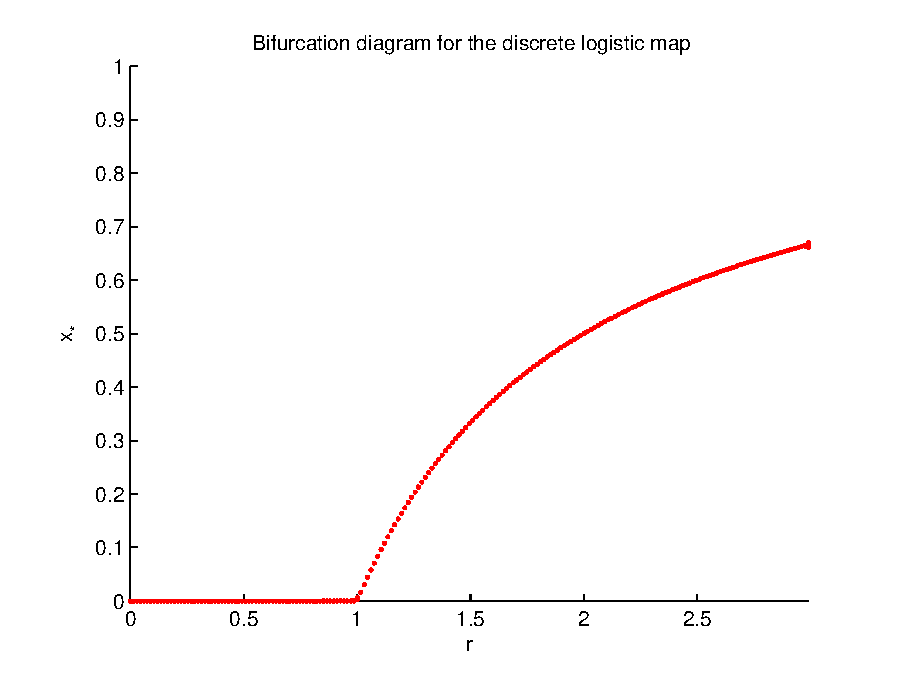
\includegraphics[width=0.5\textwidth]
{../figs_02_population_growth/bif_cascade_1}
\end{center}

\vskip0.5cm
\noindent{\bf Conclusion 2.} Building upon {\bf Conclusion 1}, we therefore deduce that
\begin{itemize}
\item if $r\in(0,1)$, then $x=0$ is attracting, and the fixed point $x=p$ does not exist,
\item if $r\in(1,3)$, then $x=0$ is repelling, and the fixed point $x=p$ exists and is attracting,
\item if $r>3$, then $x=0$ is repelling, and the fixed point $x=p$ exists and is repelling.
\end{itemize}


\begin{remark}
A fixed point that is such that $|f'(p)|\neq 1$, or a periodic point such that $|(f^k)'(p)|\neq 1$, is called \emph{hyperbolic}. In the case that $|f'(p)|=1$, or, for a periodic point, $|(f^k)'(p)|=1$, then $p$ is called \emph{non hyperbolic}. The non hyperbolic case is harder to treat. Here, the case $r=1$ is a \emph{non hyperbolic} case. However, the probability that $r=1$ is zero (the set $r=\{1\}$ has measure zero in the parameter domain $0<r<4$), explaining why, most of the time, the case of $r$ taking a single value, such as $r=1$, is omitted.
\end{remark}



\subsection{Stable sets of the fixed points}
{\bf Conclusion 2} establishes that $x=0$ and $x=p$ are attracting when, respectively, $r\in(0,1)$ and $r\in(1,3)$. This is not sufficient to characterize the behavior of all solutions. Remember that attractiveness of a fixed point $x^*$ implies that there is a neighborhood of $x^*$ that belongs to $W^s(x^*)$, i.e., there exists 
a neighborhood $\mathcal{N}\ni x^*$ such that $\forall x\in\mathcal{N}$, $x$ is forward asymptotic to $x^*$.

If we want to make sure that we have the ``complete picture'', we need to show that $W^s(x^*)=[0,1]$, i.e., that all solutions go to $x^*$. There are several ways to tackle this problem, only one is shown here.

\subsubsection{Case of the fixed point $x=0$ (i.e., case $0<r<1$)}
Since $r<1$, it follows that $f_r(x)=r x(1-x)<x(1-x)$ Also, $x\in[0,1]$ implies that $1-x\in[0,1]$, and therefore $f_r(x)<x(1-x)\leq x$. Therefore, for any $x_0\in[0,1]$,
\begin{align*}
x_1 &= f_r(x_0) \\
&< x_0 \\
x_2 &= f_r(x_1) \\
& < x_1.
\end{align*}
Therefore we have a strictly decreasing sequence. Since $[0,1]$ is invariant, the sequence is bounded below by $0$. Therefore $\lim_{k\to\infty}f^k(x_0)=0$, and $W^s(0)=[0,1]$ when $0<r<1$. Therefore we can strengthen {\bf Conclusion 2}.

\noindent{\bf Conclusion 3$'$.} If $0<r<1$, then for all $x_0\in[0,1]$, $\lim_{k\to\infty}f^k(x_0)=0$, or, equivalently, $\lim_{t\to\infty}x_t=0$.

\begin{remark}
In the considerations above, we could have used Theorem~\ref{th:gas_1} directly, once it was established that $f_r(x)<x$.
\end{remark}
 

\subsubsection{Case of the fixed point $x=p$ (i.e., case $1<r<3$)}
We know that $f_r$ is increasing from a minimum of 0 at $x=0$ to a maximum $r/4$ at $x=1/2$, and then decreasing from there to a minimum of 0 at $x=1$. Therefore, we must distinguish two cases: $r<2$ and $r>2$.


\paragraph{Case $1<r<2$}
In the case $r<2$, the intersection of $f_r(x)$ with the first bisectrix $x$ occurs before the maximum $r/4$ is reached (see Figure~\ref{fig:logistic_1dot5}).
\begin{figure}[htbp]
\begin{center}
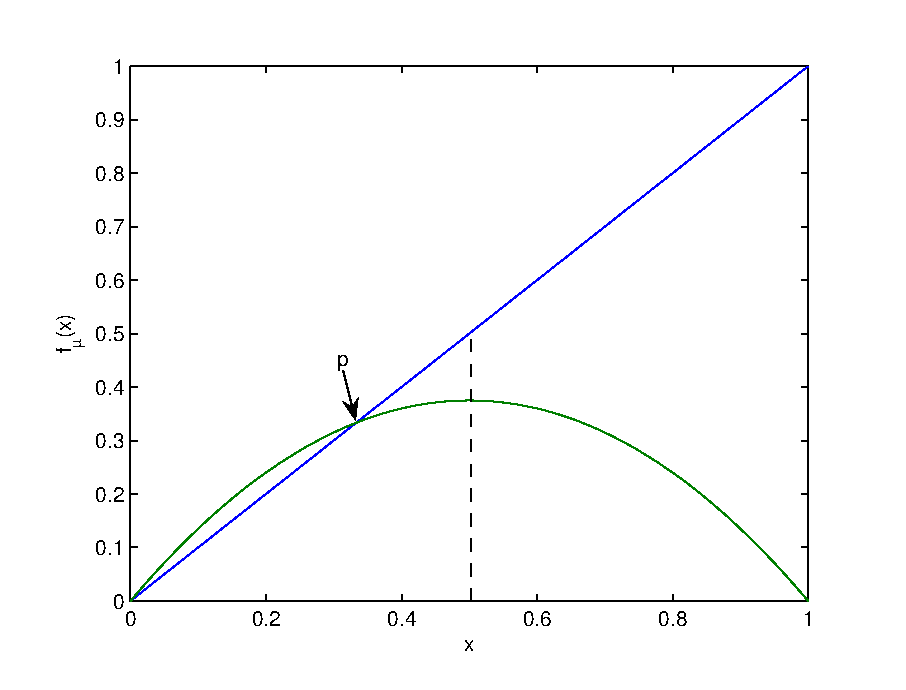
\includegraphics[width=0.5\textwidth]{../figs_02_population_growth/logistic_1dot5}
\end{center}
\caption{The function $f_{1.5}(x)$.}\label{fig:logistic_1dot5}
\end{figure}
Then we are in a position to use part {\bf a} in Theorem~\ref{th:FP_gas_discrete_4}, giving the conclusion.

\paragraph{Case $2<r<3$}
In the case $r>2$, the intersection of $f_r(x)$ with the first bisectrix $x$ occurs after the maximum $r/4$ is reached (see Figure~\ref{fig:logistic_2dot5}).
\begin{figure}[htbp]
\begin{center}
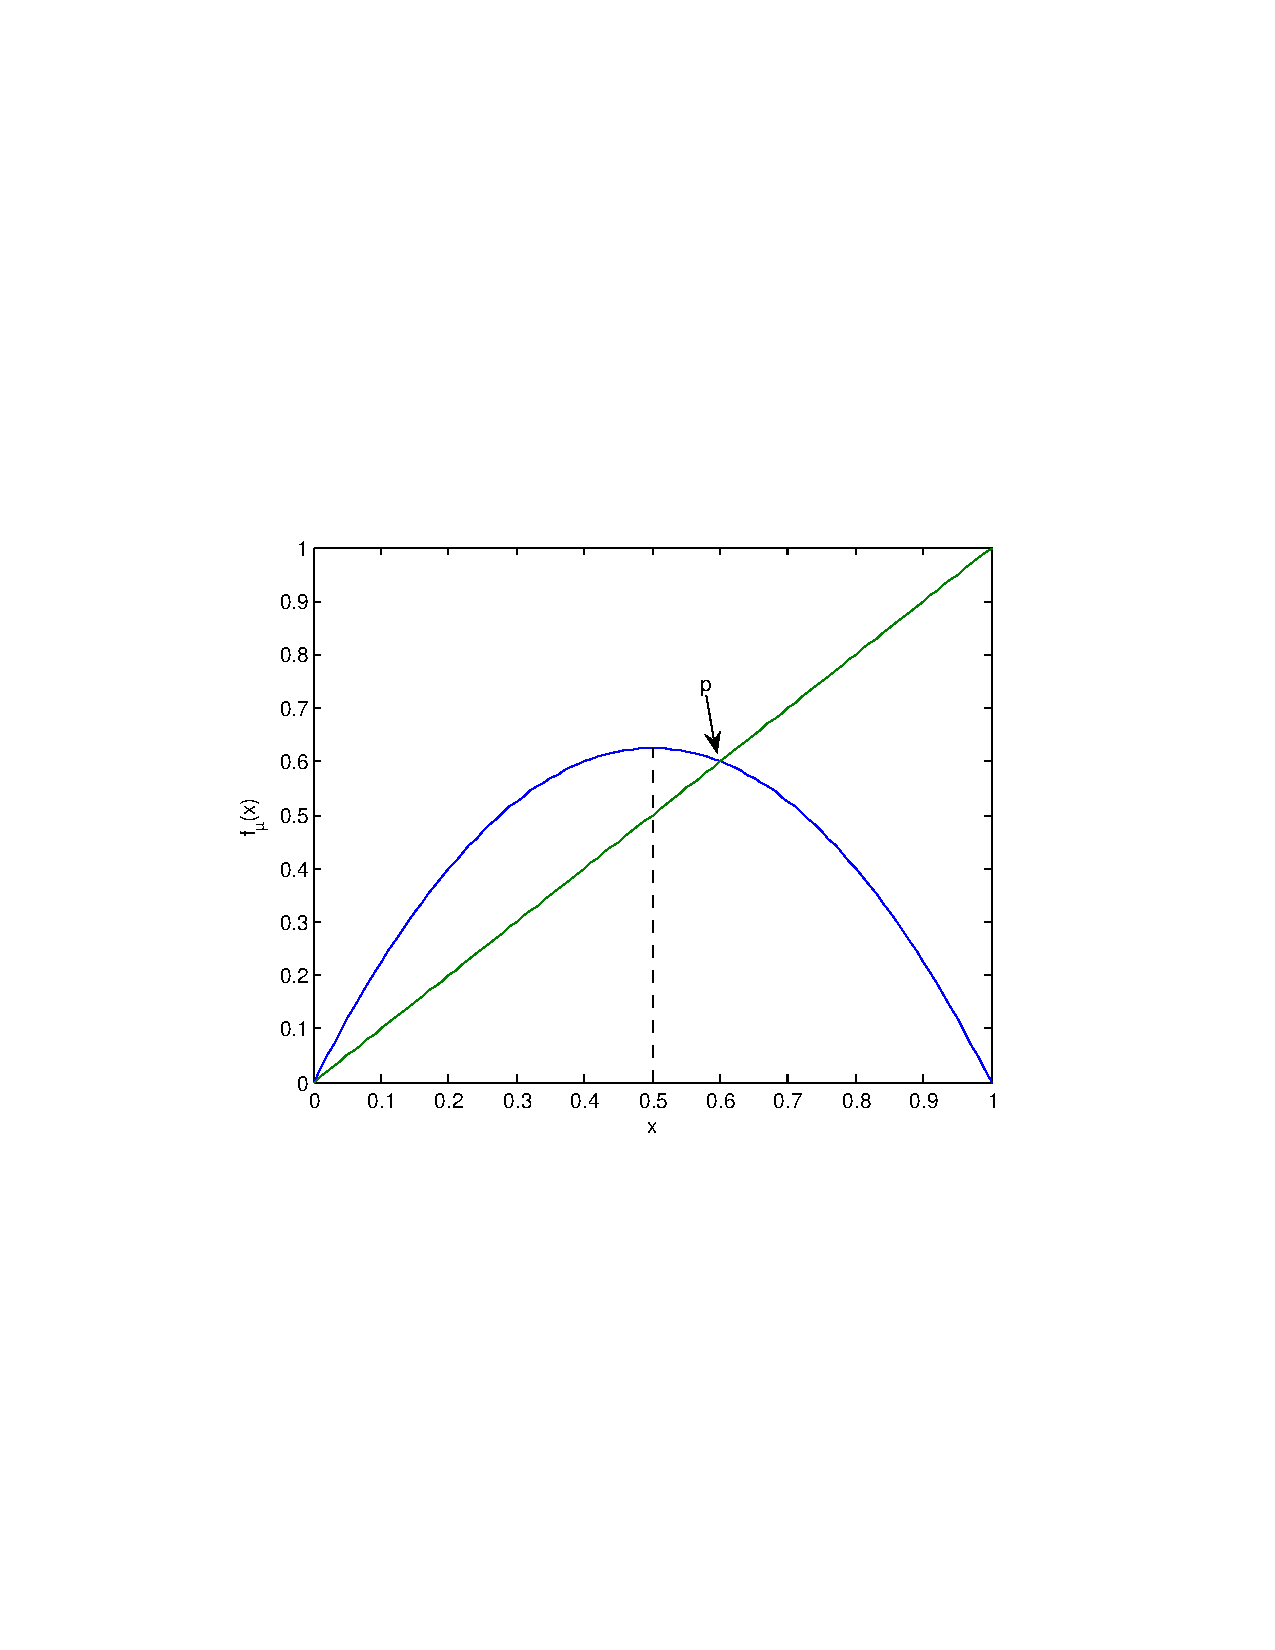
\includegraphics[width=0.5\textwidth]{../figs_02_population_growth/logistic_2dot5}
\end{center}
\caption{The function $f_{2.5}(x)$.}\label{fig:logistic_2dot5}
\end{figure}
We use Theorem~\ref{th:gas_2} in Appendix~\ref{sec:global_stability}. In order to be able to apply this theorem, we must first prove that there are no 2-cycles. For this purpose, we could try to use Theorem~\ref{th:no_cycles}, but it fails to provide the conclusion here. Here, we can use the result from Section~\ref{sec:2cycles}, where it is shown by explicit calculation that there are no 2-cycles for $r<3$.
It is clear that $f$ satisfies the hypotheses of Theorem~\ref{th:gas_2}. Indeed, $f$ is decreasing for $x>1/2$.

\begin{remark}
We could also have used part {\bf b} in Theorem~\ref{th:FP_gas_discrete_4}, but this required to show that $f^2(x)>x$ for $x\in(1/2,p)$.
\end{remark}

{\bf Global stability}
By theorem \ref{th:FP_gas_discrete_4} the equilibrium $p$ is globally asymptotically stable for $1<\mu<3$.


\paragraph{Case $r=2$}
The result used to treat the case $r<2$ can, in the present case, be extended to include the case where $r=2$.


% Here, the first idea would be to show the following:
% \begin{itemize}
% \item if $x_0\in(0,p)$, then $\{x_k\}$ is an increasing sequence,
% \item if $x_0\in(p,1)$, then $\{x_k\}$ is a decreasing sequence.
% \end{itemize}
% Note, however, that this is not sufficient: clearly, nothing forbids the sequence from ``jumping'' from one side of $p$ to the other. This is easy to see using cobwebbing: choosing $x_0$ such that $f_\mu(x_0)>p$ is not difficult (if suffices to choose $x_0$ such that $f_\mu(x_0)$ is above the line $y=p$). We thus want to show that the jumps take us closer and closer to $p$.
% 
% To do this, we consider the interval $I_0=(\varepsilon,1)$, with $\varepsilon>0$ small. We have $f_\mu'(0)=\mu>1$, and by continuity of $f_\mu'$, it is therefore possible to choose $\varepsilon$ small enough that $f_\mu'(\varepsilon)=\mu(1-2\varepsilon)>1$.



\subsection{Existence of points of period 2}
\label{sec:2cycles}
We now study the existence of periodic points with least period 2, that is, fixed points of the map $f_r^2(x)$. We have
\begin{align}
f_r^2(x) &= f_r(f_r(x)) \nonumber\\
&= r f_r(x)(1-f_r(x)) \nonumber\\
&= r^2 x(1-x)(1-r x(1-x)). \label{eq:f_mu_2_a}
\end{align}
Remark that 0 and $p$ are points of period 2. Indeed, a fixed point $x^*$ of $f$ satisfies $f(x^*)=x^*$, and as a consequence, $f^2(x^*)=f(f(x^*))=f(x^*)=x^*$. This is extremely helpful in localizing the other periodic points, if there are any. Indeed, writing the fixed point equation as
\[
f_r^2(x)-x=0,
\]
and defining $Q(x):=f_r^2(x)-x$, we see that, since $0$ and $p$ are fixed points of $f_r^2$, they are roots of $Q(x)$. Therefore, $Q$ can be factorized as
\[
Q(x)=x(x-p)(-r^3x^2+Bx+C),
\]
since it is clear from \eqref{eq:f_mu_2_a} that $f_r^2$ is a polynomial of degree 4 with leading coefficient equal to $-r^3$. Substituting the value $(r-1)/r$ for $p$ in $Q$, developing $Q$ and \eqref{eq:f_mu_2_a} and equating coefficients of like powers gives
\begin{equation}\label{eq:Q}
Q(x)=x\left(x-\frac{r-1}{r}\right)\left(-r^3 x^2+r^2(r+1)x-r(r+1)\right).
\end{equation}
The roots of \eqref{eq:Q} are the fixed points of $f_r^2$. Since $x=0$ and $x=p$ are already known, we can concentrate on the roots of the polynomial
\[
R(x):=-r^3 x^2+r^2(r+1)x-r(r+1).
\]
The discriminant is $\Delta=r^4(r+1)^2-4r^4(r+1)=r^4(r+1)(r+1-4)=r^4(r+1)(r-3)$. Therefore, $R$ has no real root if $r<3$, a double real root if $r=3$ and distinct real roots if $r>3$. We want real valued solutions, so discard the case $r<3$. In the case $r=3$, the root is
\[
\left.\frac{r+1}{2r}\right|_{r=3}=\frac 23,
\]
which is the value of $p$ when evaluated at $r=3$: the fixed point $p$ and the fixed point deduced from $R$ coincide at $r=3$.

So we now consider the case $r>3$. In this case, $R$ has two distinct real roots (that is, $f_r^2$ has two distinct real fixed points) given by
\[
\bar x_{1,2}=\frac{r+1\pm\sqrt{(r+1)(r-3)}}{2r}.
\] 
First, remark that for $r>3$ but very close to 3, it follows from the continuity of $R$ that the roots are very close to the double root $2/3$, and hence are in $(0,1)$.
More than the actual value of the roots, what is of interest at this point is to determine whether they remain in $(0,1)$ for all values of $3<r<4$.
If a root is not in $(0,1)$, it is considered to be non biologically relevant and therefore is ignored.

To show that the roots remain in $(0,1)$ as we move away from 3, we could proceed directly using the expression for $\bar x_{1,2}$. Instead, we use Descartes' rule of signs (Theorem~\ref{th:descartes}, Appendix~\ref{sec:descartes}). For this, remark that $R$ has signed coefficients $-+-$, giving two sign changes and the possibility of 0 or 2 positive real roots. On the other hand, $R(-x)$ has signed coefficients $---$, hence there are no negative real roots. As we are in the case where the roots are real, it follows that both roots are positive.

To show that the roots are also smaller than 1, consider the change of variables $z=x-1$. The polynomial $R$ is transformed into 
\begin{align*}
R_2(z) &= -r^3 (z+1)^2+r^2(r+1)(z+1)-r(r+1) \\
&= -r^3z^2+r^2(1-r)z-r.
\end{align*}
For $r>1$, all the coefficients of this polynomial are negative, implying that $R_2$ has no root $z>0$, implying in turn that $R$ has no root $x>1$.
\begin{figure}[htbp]
\begin{center}
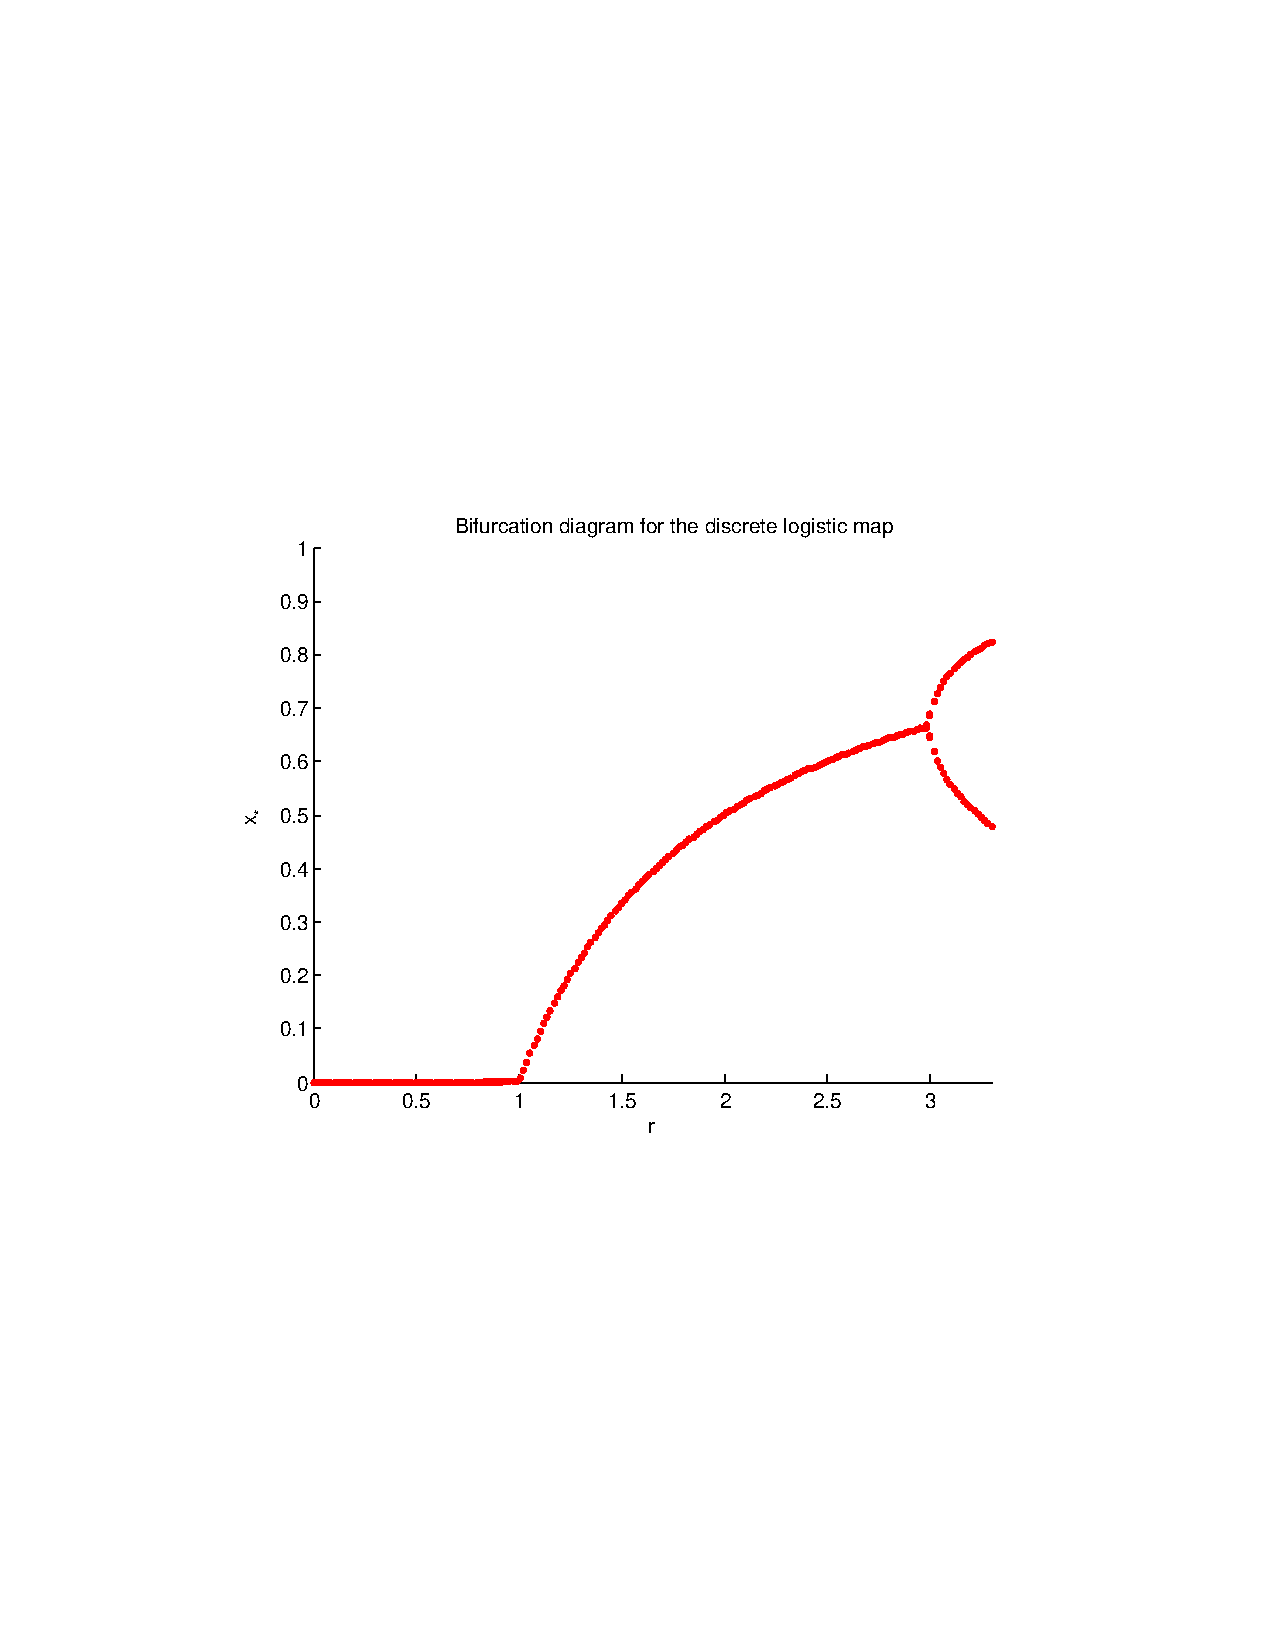
\includegraphics[width=0.5\textwidth]
{../figs_02_population_growth/bif_cascade_3}
\caption{Bifurcation diagram for the discrete logistic map showing the birth of the fixed point at $r=1$ and of the 2-cycle at $r=3$.}
\end{center}
\end{figure}


\subsection{Attractiveness of the periodic orbit}
We use Theorem~\ref{th:} which states that the $2-$cycle is locally asymptotically stable if
\[
|f_r'(\bar x_1)f_r'(\bar x_2)|<1.
\]
From \eqref{eq:dlogistic_map}, we obtain
\begin{align*}
|f_r'(\bar x_1)f_r'(\bar x_2)|
&=\left|
\left(r-(r+1)+\sqrt{(r+1)(r-3)}\right)
\left(r-(r+1)-\sqrt{(r+1)(r-3)}\right)
\right| \\
&=\left|
\left(1+\sqrt{(r+1)(r-3)}\right)
\left(1-\sqrt{(r+1)(r-3)}\right)
\right|.
\end{align*}
Therefore,
\begin{align*}
|f_r'(\bar x_1)f_r'(\bar x_2)|<1 &\Leftrightarrow |1-(r+1)(r-3)|<1 \\
&\Leftrightarrow -1<1-(r+1)(r-3)<1 \\
&\Leftrightarrow 0<(r+1)(r-3)<2.
\end{align*}
Evidently, the inequality $0<(r+1)(r-3)$ is satisfied if $r>3$. On the other hand, the quadratic inequality $(r+1)(r-3)<2$ is satisfied if $r<1+\sqrt{6}$.
Therefore, the 2-cycle is locally asymptotically stable if 
\[
3<r<1+\sqrt{6}
\]
and unstable if $r>1+\sqrt{6}$.






\subsection{The cascade of bifurcation to chaos}
\label{sec:chaos}
We have seen that at $r=1$, $r=3$ and $r=1+\sqrt{6}$, there are changes in the stability of the various equilibria that are present, and that additional equilibria can be born. These values of $r$ are called \textbf{bifurcation points}. 

The first bifurcation that occurs, at $r=1$, is different in nature from the ones that follow. It is called a \textbf{transcritical bifurcation}, and corresponds to an exchange of stability between zero and $p$ (recall that although $p$ is not relevant for $r<1$, it still does exist). 

Subsequent bifurcations are called \textbf{period-doubling bifurcations}. By continuing the analysis of the logistic map, we see that it undergoes a a sequence of period doubling bifurcations, called the \textbf{period-doubling cascade}, as $r$ increases from 3 to 4 (see Figure~\ref{fig:bif_cascade_29_4}):
\begin{itemize}
\item for $1+\sqrt{6}<r<3.5441$ there is a stable $4-$cycle, followed by a period doubling at $r=3.5441$;
\item for $3.5441<r<3.5644$ there is a stable $8-$cycle, followed by a period doubling at $r=3.5644$;
\item for $3.5644<r<3.5688$ there is a stable $16-$cycle, followed by a period doubling at $r = 3.5688$;
\item $\ldots$ other stable cycles of increasing period $2^n$;
\item finally, for $r> 3.57$, a cycle of period $3$ exists. In that case, the solutions are called \textbf{chaotic} (see below).
\end{itemize}
\begin{figure}[htbp]
\begin{center}
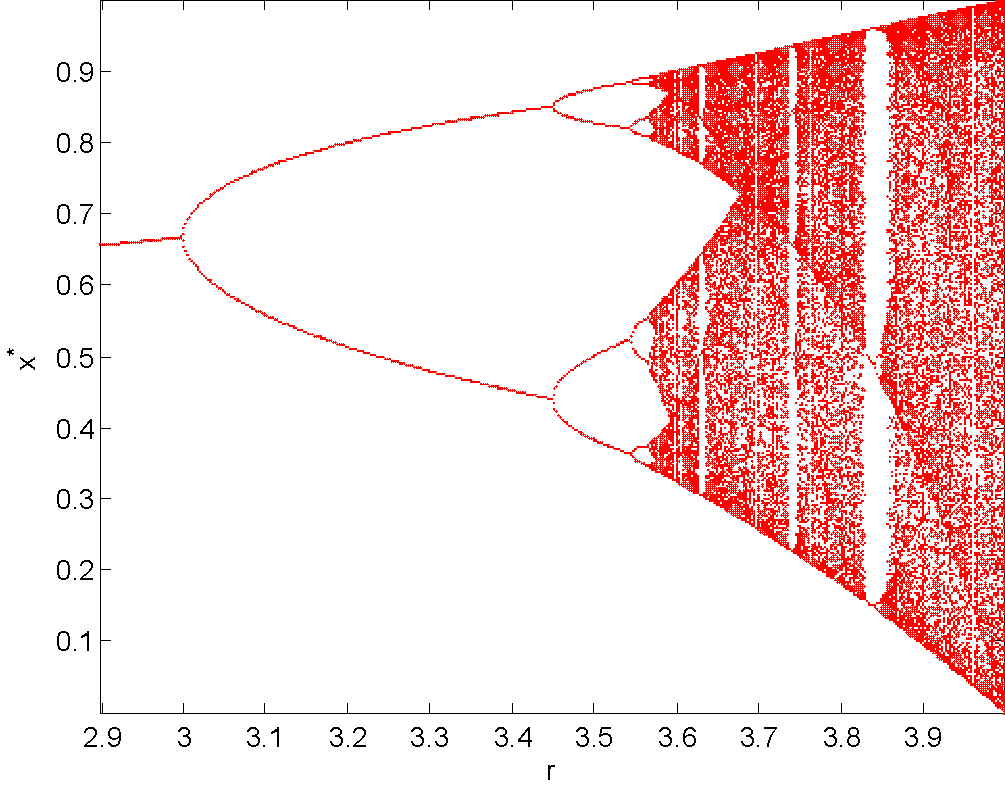
\includegraphics[width=0.6\textwidth]
{../figs_02_population_growth/cascade_29_4}
\caption{Bifurcation cascade for $2.9\leq r\leq 4$.}
\label{fig:bif_cascade_29_4}
\end{center}
\end{figure}
The points at which the period doublings occur has a very interesting (and intriguing) property:
The bifurcation points form a sequence, $\{r_n\}$, that has the property that
\[
\lim_{n\to\infty}\frac{r_n-r_{n-1}}{r_{n+1}-r_n}
\]
exists and is a constant, called the Feigenbaum constant, equal to 4.669202\ldots
This constant has been shown to be the same in many of the maps that undergo the same type of cascade of period doubling bifurcations.

To finish, let us briefly discuss chaos. Note that the mathematics are quite involved and well beyond the scope of these notes.
Denoting $\triangleright$ an order symbol, Sharkovskii's ordering of integers is as follows:
\begin{gather*}
3\triangleright 5\triangleright 7 \triangleright 9 \triangleright 11\triangleright \cdots \triangleright 2\cdot 3\triangleright  2\cdot 5\triangleright \cdots \triangleright 2\cdot 9\triangleright\cdots\triangleright 2^2\cdot 3\triangleright 2^2\cdot 5\triangleright \cdots \\
\triangleright 2^n\cdot 3\triangleright 2^n\cdot 5\triangleright \cdots\triangleright 2^{n+1}\cdot 3\triangleright 2^{n+1}\cdot 5\triangleright \cdots
\triangleright 2^{n+1}\triangleright 2^n\triangleright \cdots 2^2 \triangleright 2\triangleright 1.
\end{gather*}
This gives an ordering of all positive integers. The following result helps characterizing the behavior of the cascade.
\begin{theorem}[Sharkovskii]\label{th:sharkovskii}
Let $f:I\subset\IR\to\IR$ be a continuous function. Assume that $f$ has a point of least period $n$ and $n\triangleright k$. Then $f$ has a point of least period $k$.
\end{theorem}


\begin{figure}[htbp]
\begin{center}
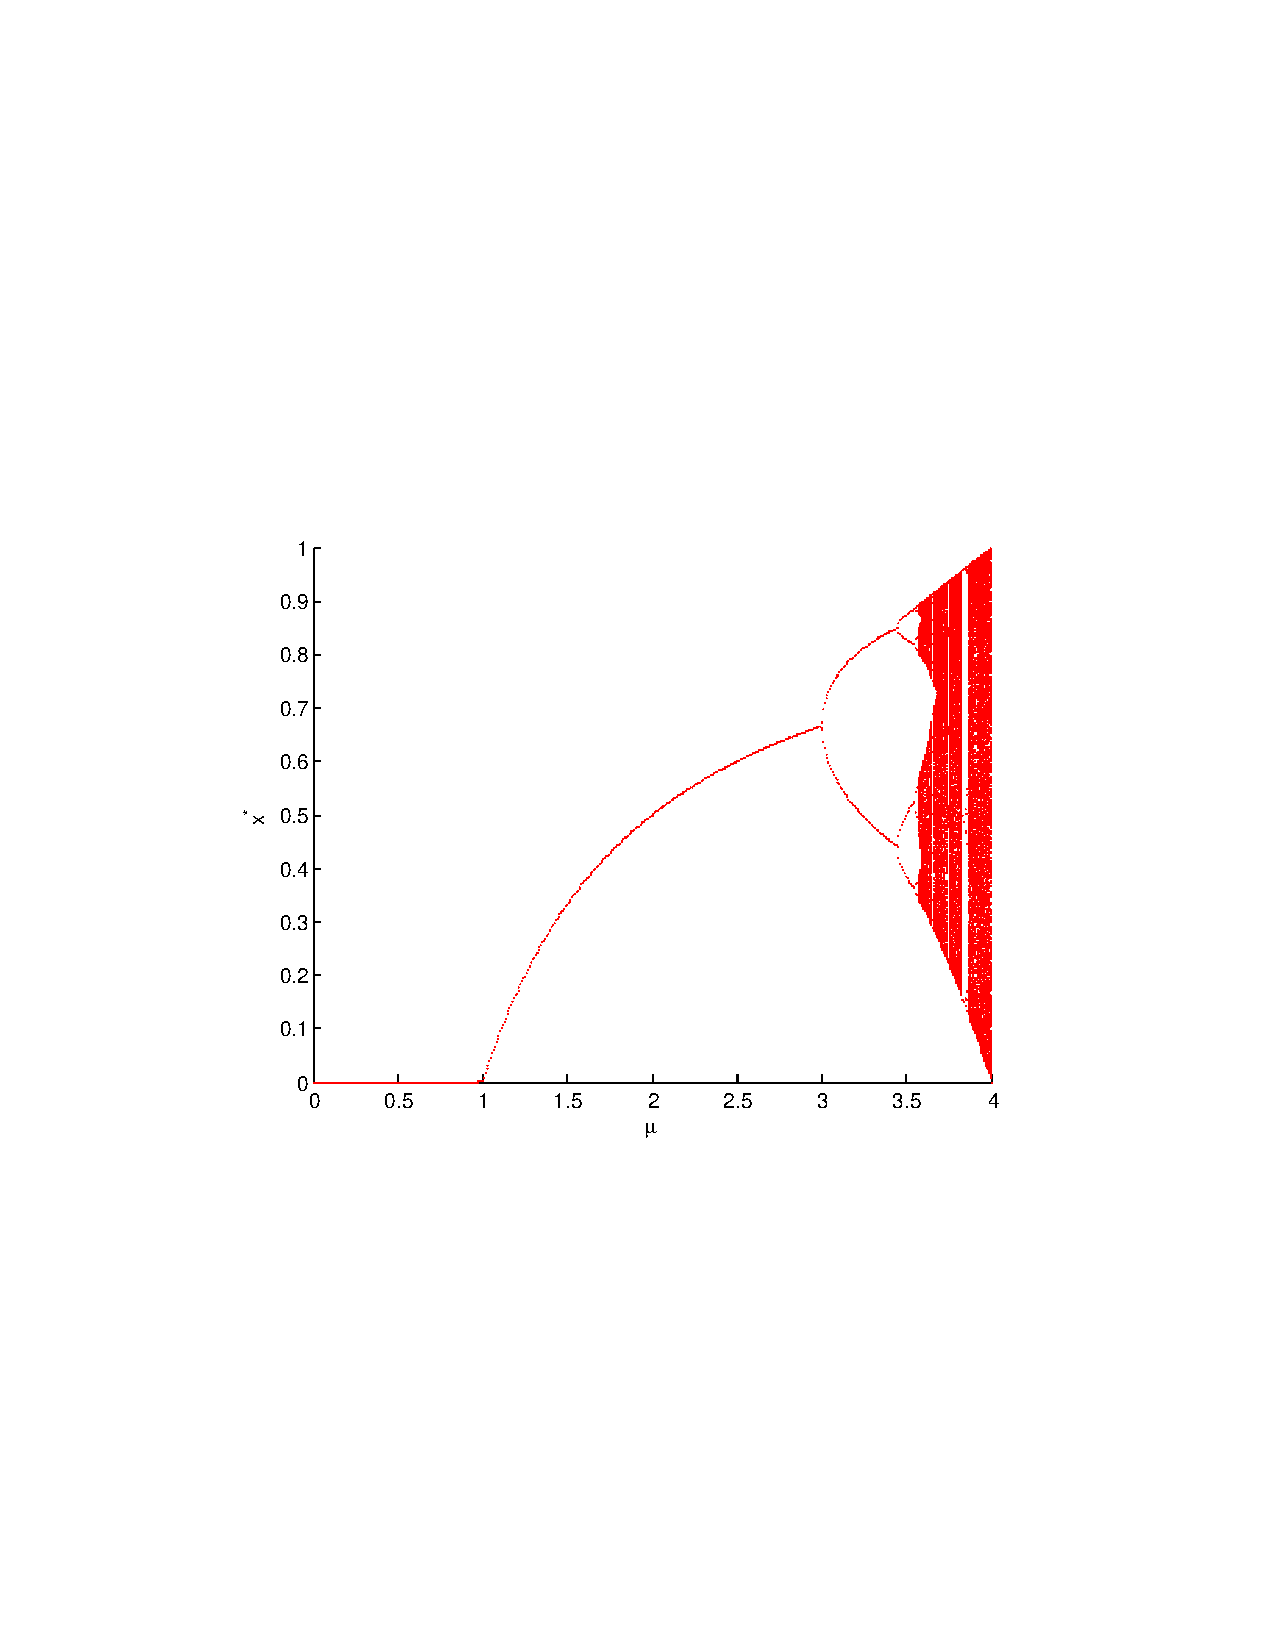
\includegraphics[width=0.5\textwidth]
{../figs_02_population_growth/analysis_logistic_cascade_full}
\end{center}
\caption{The cascade of bifurcation to chaos for the logistic map.}
\end{figure}

We have seen that for $r>3.57$, there is a cycle of period 3 for the logistic map. By Sarkovskii's theorem, the presence of period 3 points implies the presence of points of all periods.
At this point, the system is said to be in a \textbf{chaotic regime}, or \textbf{chaotic}.




\section{Conclusion}

We have used three different modelling paradigms to describe the growth of a population in a \textbf{logistic} framework:
\begin{itemize}
\item The ODE version of Section~\ref{sec:ODE_logistic} has monotone solutions converging to the carrying capacity $K$.
\item The DDE version of Section~\ref{sec:DDE_logistic} has oscillatory solutions, either converging to $K$ or, if the delay is too large, periodic about $K$.
\item The discrete time version of Section~\ref{sec:DE_logistic} has all sorts of behaviors, and can be chaotic.
\end{itemize}
It is important to be aware that the {\bf choice of modelling method} is almost {\bf as important} in the outcome of the model as the precise formulation/hypotheses of the {\bf model}.


%\section{Critic of the logistic equation in the US census case}
%
%\frame{\frametitle{What is wrong with the logistic equation here?}
%\begin{itemize}
%\item The carrying capacity is constant.
%\item The model does not take immigration into account (for the US, this is an important component).
%\end{itemize}
%}
%
%
%\section{Population curves -- Gompertz}
%
%\frame{
%\begin{center}
%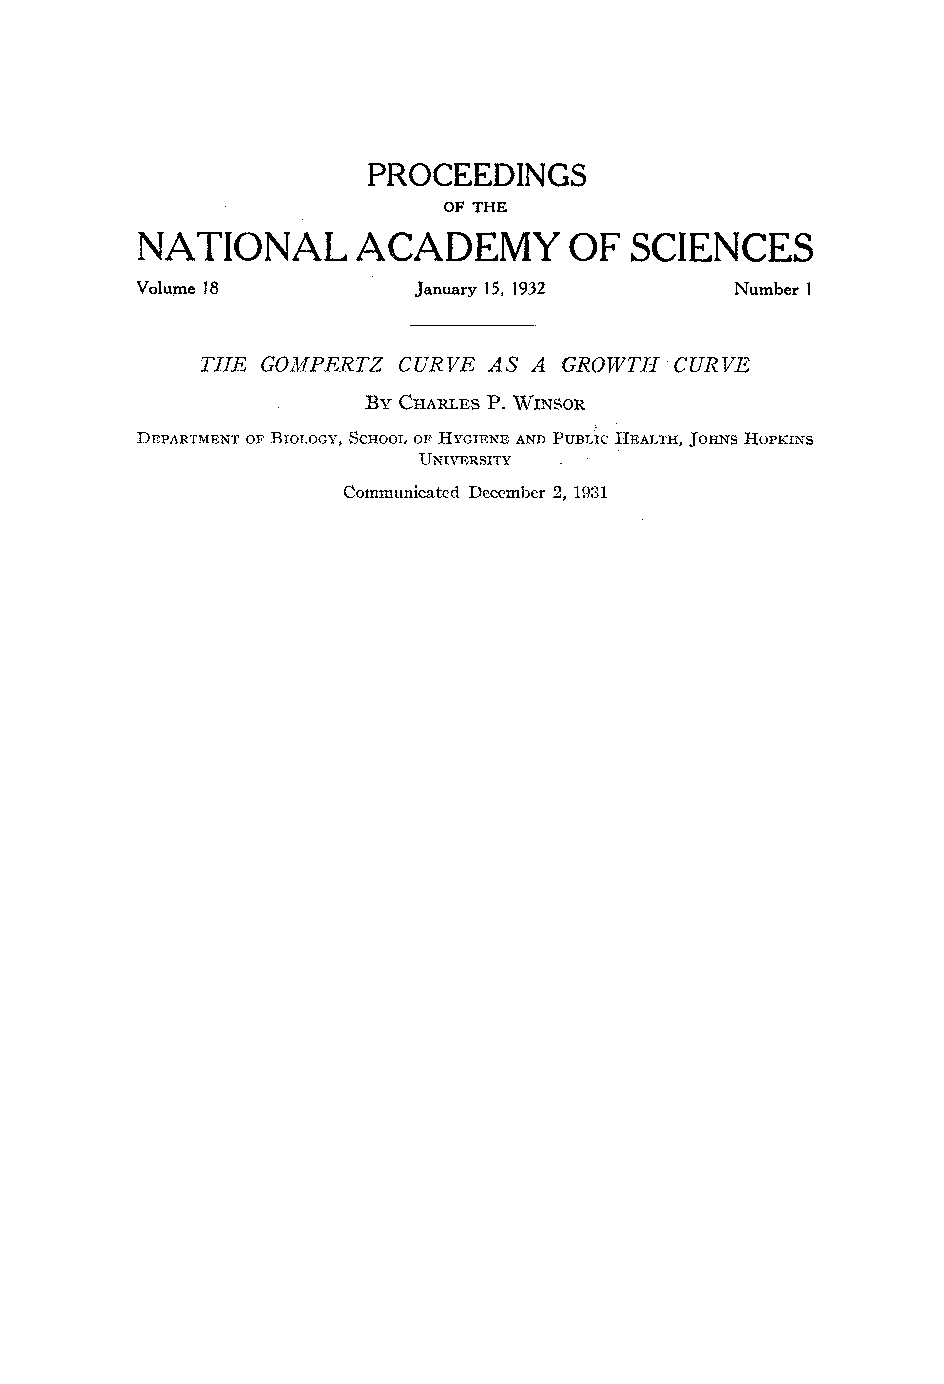
\includegraphics[width=0.95\textwidth]{title_Winsor1932PNAS18}
%\end{center}
%}
%
%\frame{
%\begin{center}
%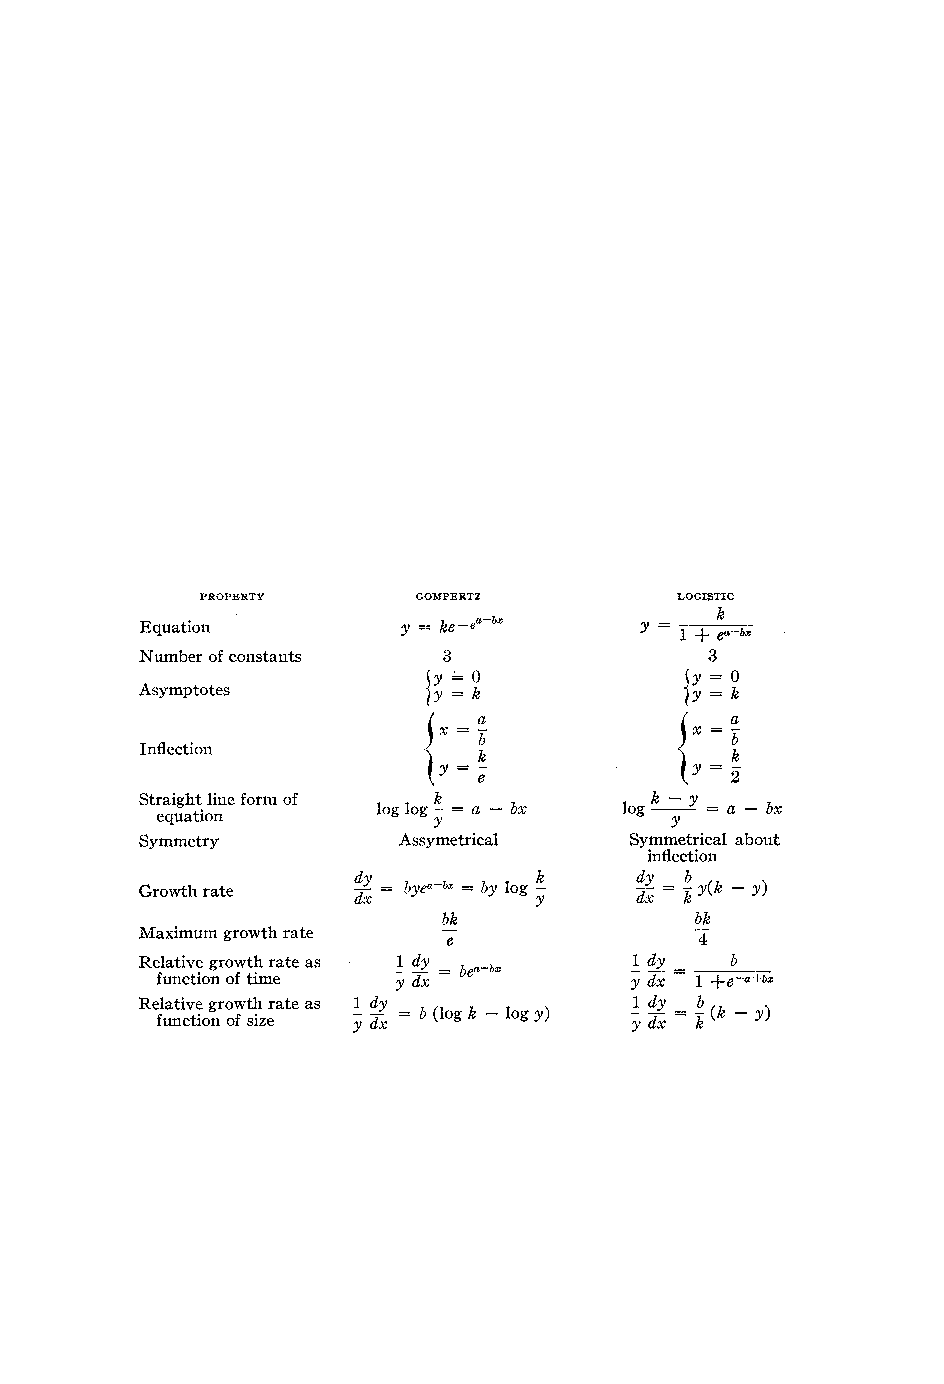
\includegraphics[width=0.95\textwidth]{table_Winsor1932PNAS18}
%\end{center}
%}
%
